

\documentclass{beamer}
\usepackage[utf8]{inputenc}
\usepackage{url}
\usepackage{algorithm}
\usepackage{algpseudocode}
\usepackage{lmodern}
\usepackage{natbib}
\usepackage{tikz}
\usepackage{physics}
\usepackage{graphicx} % Allows including images
\graphicspath{ {./images/} }
\usepackage{booktabs} % Allows the use of \toprule, \midrule and \bottomrule in tables
\usepackage{tikz}
\usetikzlibrary{arrows.meta}

\usetikzlibrary{mindmap, trees, shadows, shapes, calc, fadings, positioning, decorations.pathreplacing, intersections, shapes, arrows}

%\usetheme{Hannover}
%\usecolortheme{spruce}
% EPIC FAIL
\usetheme{default}
%\usecolortheme{beetle}
\usepackage{graphics}

\usepackage{color}
\definecolor{new_turquoise}{RGB}{40,151,158}%{251,190,94}
\setbeamercolor{title}{fg=new_turquoise}


\usepackage{hyperref}
\hypersetup{colorlinks=true, urlcolor=blue}

%[colorlinks=true, urlcolor=blue, linkcolor=red]{hyperref}


\makeatletter
\setbeamertemplate{frametitle}{
    \ifbeamercolorempty[bg]{frametitle}{}{\nointerlineskip}%
    \@tempdima=\textwidth%
    \advance\@tempdima by\beamer@leftmargin%
    \advance\@tempdima by\beamer@rightmargin%
    \vspace*{0.8cm} 
    %\hspace*{-3cm}
    %%%%%%%%%%%%% For example insert shift to right
    \begin{beamercolorbox}[sep=0.3cm,center,wd=\the\@tempdima]{frametitle}
        \usebeamerfont{frametitle}%
        \vbox{}\vskip-1ex%
        \if@tempswa\else\csname beamer@ftecenter\endcsname\fi%
        \strut\insertframetitle\strut\par%
        {%
            \ifx\insertframesubtitle\@empty%
            \else%
            {\usebeamerfont{framesubtitle}\usebeamercolor[fg]{framesubtitle}\insertframesubtitle\strut\par}%
            \fi
        }%
        \vskip-1ex%
        \if@tempswa\else\vskip-.3cm\fi% set inside beamercolorbox... evil here...
    \end{beamercolorbox}%
}
\makeatother

\setbeamercolor{frametitle}{fg=new_turquoise}
\setbeamertemplate{itemize item}{\color{new_turquoise}$\blacksquare$}
\setbeamertemplate{itemize subitem}{\color{new_turquoise}$\blacksquare$}


% --- ENUMERATE ITEMS ---
\setbeamertemplate{enumerate item}{\color{new_turquoise}\insertenumlabel}
\setbeamertemplate{enumerate subitem}{\color{new_turquoise}\insertsubenumlabel}

\setbeamertemplate{caption}{\raggedright\insertcaption\par}

% --- COLOR THE TABLE OF CONTENTS ENTRIES ---
\setbeamercolor{section in toc}{fg=new_turquoise}
\setbeamercolor{subsection in toc}{fg=new_turquoise}
\setbeamercolor{subsubsection in toc}{fg=new_turquoise}



\usebackgroundtemplate{
    
\includegraphics[width=\paperwidth,height=\paperheight]{figs/slide-title.jpg}
} 

\title{\fontsize{49}{7.2}{\bf Fundamental Algorithmic Techniques XI}}
%\author{JW}
\date{\color{new_turquoise}\today}
%S\titlegraphic{\includegraphics[width=2cm]{figs/jw.png}}

\begin{document}
\frame{\titlepage}
%% SLIDE 1 - INTRO TO THE TEAM
%%%%%%%%%%%%%%%%%%%%%%%%%%%%%%%%%%%%%%%%%%%%%%%%%%%%%

\usebackgroundtemplate{
    
\includegraphics[width=\paperwidth,height=\paperheight]{figs/slide-pages}
} 


\setbeamertemplate{subsection in toc}{
  \color{new_turquoise}$\blacksquare$\color{black}~~\inserttocsubsection
}


% Outline frame
\begin{frame}{Outline}
    \tableofcontents
\end{frame}





\section{Linear Programming: Examples}


\begin{frame}{Linear Programming: Examples}
Formulation of Optimisation Problems with constraints:

\vspace{0.3cm}
\begin{columns}[T]
\begin{column}{0.48\textwidth}
\textbf{Example 1: Bakery Production}
\begin{itemize}
    \item \textbf{Decision Variables:} \\ $x$ = croissants, $y$ = muffins
    \item \textbf{Objective:} $\max \text{ Profit} = 3x + 4y$
    \item \textbf{Constraints:}
    \[
    \begin{aligned}
    2x + 3y &\leq 100 \quad \text{(Flour)}\\
    x + 2y &\leq 50 \quad \text{(Sugar)}\\
    3x + 2y &\leq 80 \quad \text{(Labor)}\\
    x, y &\geq 0
    \end{aligned}
    \]
\end{itemize}
\end{column}


\begin{column}{0.48\textwidth}
\textbf{Example 2: Manufacturing}
\begin{itemize}
    \item \textbf{Decision Variables:} \\ $b$ = basic product, $p$ = premium product
    \item \textbf{Objective:} $\max P = 30b + 40p$
    \item \textbf{Constraints:}
    \[
    \begin{aligned}
    20b + 30p &\leq 3900 \quad \text{(Res 1)}\\
    15b + 30p &\leq 3300 \quad \text{(Res 2)}\\
    b, p &\geq 0
    \end{aligned}
    \]
\end{itemize}
\end{column}
\end{columns}
\end{frame}



\begin{frame}{Transportation Problem: Example}
\tiny %footnotesize  % Reduce base font size for entire frame content

\textbf{Cost Matrix, Supply \& Demand}
\vspace{0.1cm}
\begin{center}
\scriptsize  % Even smaller for the dense table
\begin{tabular}{c|cccc|c}
     & $D_1$ & $D_2$ & $D_3$ & $D_4$ & Supply \\ \hline
$S_1$ & 19 & 30 & 50 & 10 & 7 \\
$S_2$ & 70 & 30 & 40 & 60 & 9 \\
$S_3$ & 40 & 8  & 70 & 20 & 18 \\ \hline
Demand & 5  & 8  & 7  & 14 & \textbf{34}
\end{tabular}
\end{center}

\vspace{0.2cm}
\textbf{LP Formulation:}
\begin{itemize}
    \item \textbf{Decision Variables:} $x_{ij}$ = units shipped from $S_i$ to $D_j$ \quad $(i=1,2,3;\; j=1,2,3,4)$
    \item \textbf{Objective:} 
    \[
    \scriptsize  % Smaller font for long objective equation
    \min Z = 19x_{11} + 30x_{12} + 50x_{13} + 10x_{14} + 70x_{21} + 30x_{22} + 40x_{23} + 60x_{24} + 40x_{31} + 8x_{32} + 70x_{33} + 20x_{34}
    \]
\end{itemize}

\vspace{-0.2cm}  % Save vertical space
\begin{columns}[T]
\begin{column}{0.48\textwidth}
\textit{Supply Constraints:}
\[
\scriptsize
\begin{aligned}
x_{11} + x_{12} + x_{13} + x_{14} &= 7 \\
x_{21} + x_{22} + x_{23} + x_{24} &= 9 \\
x_{31} + x_{32} + x_{33} + x_{34} &= 18
\end{aligned}
\]
\end{column}
\begin{column}{0.48\textwidth}
\textit{Demand Constraints:}
\[
\scriptsize
\begin{aligned}
x_{11} + x_{21} + x_{31} &= 5 \\
x_{12} + x_{22} + x_{32} &= 8 \\
x_{13} + x_{23} + x_{33} &= 7 \\
x_{14} + x_{24} + x_{34} &= 14
\end{aligned}
\]
\end{column}
\end{columns}
\vspace{-0.1cm}
\centering \textbf{Non-negativity:} $x_{ij} \geq 0 \quad \forall i,j$
\end{frame}


\begin{frame}{Example: A two-variable linear program}
  \small
  \begin{columns}[T]
    % === LEFT COLUMN: Text & Formulation ===
    \begin{column}{0.5\textwidth}
      \textbf{Formulation:}
      \[
        \begin{aligned}
          \text{maximize} \quad & 2x_1 + 3x_2 \\
          \text{subject to} \quad & -x_1 + x_2 \le 8 \\
                                  & 2x_1 + x_2 \le 10 \\
                                  & 5x_1 - 2x_2 \ge -2 \\
                                  & x_1, x_2 \ge 0
        \end{aligned}
      \]
      \vspace{0.5em}
      \textbf{Key Ideas:}
      \begin{itemize}
        \item Each constraint $\rightarrow$ a half-plane
        \item Feasible region = intersection (convex polygon)
        \item Optimal solution at a \textbf{vertex}
      \end{itemize}
    \end{column}

    % === RIGHT COLUMN: Image Placeholder ===
    \begin{column}{0.5\textwidth}
      \centering
      \vspace{1em}
      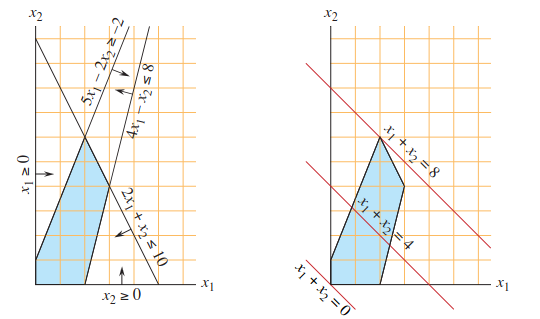
\includegraphics[width=1.1\linewidth, keepaspectratio]{figs/lp2vars.png}
      %\fbox{\parbox{3.5cm}{\centering\vspace{1.5em}\texttt{[Insert Plot]}\\{\footnotesize Feasible region \& objective}\vspace{1.5em}}}
    \end{column}
  \end{columns}
\end{frame}



\section{Primal, Dual \& Optimisation }


\begin{frame}{General Linear Programming Formulation}
  \footnotesize  % Global reduction for entire frame
  
  \textbf{Core Idea:} Optimize a linear objective subject to linear constraints.
  \textit{\scriptsize (Strict inequalities not allowed in LP.)}

  \vspace{0.15cm}

  \textbf{Standard Maximization Form:}
  \[
    \scriptsize
    \setlength{\arraycolsep}{2pt}
    \begin{aligned}
      \max \quad & Z = \sum_{j=1}^{n} c_j x_j \\
      \text{s.t.} \quad & \sum_{j=1}^{n} a_{ij} x_j \leq b_i \quad \forall i = 1,\dots,m \\
                        & x_j \geq 0 \quad \forall j = 1,\dots,n
    \end{aligned}
  \]

  \vspace{0.1cm}
  \textbf{Compact Matrix Notation:}
  \[
    \scriptsize
    \begin{aligned}
      \max \quad & \mathbf{c}^\top \mathbf{x} \\
      \text{s.t.} \quad & \mathbf{A}\mathbf{x} \leq \mathbf{b} \\
                        & \mathbf{x} \geq \mathbf{0}
    \end{aligned}
  \]
  \textit{\scriptsize where $\mathbf{A} \in \mathbb{R}^{m \times n}$, $\mathbf{b} \in \mathbb{R}^m$, $\mathbf{c}, \mathbf{x} \in \mathbb{R}^n$.}

  \vspace{0.1cm}
  \begin{itemize}%[leftmargin=*, nosep]
    \item \textbf{Objective:} $\mathbf{c}^\top \mathbf{x}$ — linear combo of decision variables
    \item \textbf{Constraints:} $m$ linear inequalities $+$ $n$ non-negativity bounds
    \item \textbf{Feasible Region:} Intersection of half-spaces $\Rightarrow$ convex polyhedron
  \end{itemize}
\end{frame}



\begin{frame}{Introduction to Primal / Dual Space}
  \footnotesize
  % === TOP ROW: Primal (Left) & Dual (Right) ===
  \begin{columns}[T]
    % Primal
    \begin{column}{0.48\textwidth}
      \textbf{Primal (Max)}
      \[
        \small
        \begin{aligned}
          \max \quad & 3x_1 + x_2 + 4x_3 \\
          \text{s.t.} \quad & x_1 + x_2 + 3x_3 \le 30 \\
                            & 2x_1 + 2x_2 + 5x_3 \le 24 \\
                            & 4x_1 + x_2 + 2x_3 \le 36 \\
                            & x_1, x_2, x_3 \ge 0
        \end{aligned}
      \]
    \end{column}
    % Dual
    \begin{column}{0.48\textwidth}
      \textbf{Dual (Min)}
      \[
        \small
        \begin{aligned}
          \min \quad & 30y_1 + 24y_2 + 36y_3 \\
          \text{s.t.} \quad & y_1 + 2y_2 + 4y_3 \ge 3 \\
                            & y_1 + 2y_2 + y_3 \ge 1 \\
                            & 3y_1 + 5y_2 + 2y_3 \ge 4 \\
                            & y_1, y_2, y_3 \ge 0
        \end{aligned}
      \]
    \end{column}
  \end{columns}

  % === BOTTOM ROW: Key Relationships (Full Width) ===
  %\vspace{0.8em}
  %\hrule height 0.4pt
  %\vspace{0.6em}
  \textbf{Primal–Dual Relationships:}
  \begin{itemize}
	  \item \textbf{Constraint $\leftrightarrow$ Variable:} Each primal constraint corresponds to a {\bf dual variable} ($y_i$), and vice versa.
    \item \textbf{Coefficient mapping:} The primal objective coefficients become RHS of dual constraints; primal RHS becomes dual objective coefficients.
    \item \textbf{Weak duality:} For any feasible $x$ and $y$: $\;c^\top x \le b^\top y$.
    \item \textbf{Strong duality:} If both are feasible, optimal values are equal: $\;c^\top x^* = b^\top y^*$.
    \item \textbf{Complementary slackness:} At optimum, $x_j > 0 \Rightarrow$ $j$-th dual constraint is tight, and $y_i > 0 \Rightarrow$ $i$-th primal constraint is tight.
  \end{itemize}
\end{frame}








\begin{frame}{Fundamental Theorem of Linear Programming}
  \footnotesize
  
  \textbf{Theorem} 
  Any linear program in standard form satisfies \textbf{exactly one} of the following:
  
  %\vspace{0.3cm}
  
  \begin{enumerate} %[label=\textbf{\arabic*.}, leftmargin=*, nosep]
    \item \textbf{Optimal:} Has an optimal solution with finite objective value.
    \item \textbf{Infeasible:} No point satisfies all constraints (feasible region = $\emptyset$).
    \item \textbf{Unbounded:} Feasible region is non-empty, but objective can be made arbitrarily large (for max) or small (for min).
  \end{enumerate}
  
  %\vspace{0.4cm}
  %\hrule height 0.3pt
  %\vspace{0.3cm}
  \bigskip
  \bigskip
  \bigskip

  \textbf{Implications:}
  \begin{itemize} %[leftmargin=*, nosep]
    \item Guarantees that LP solvers will terminate with a definitive answer
    \item Underpins the correctness of the simplex method and interior-point algorithms
    \item Justifies checking feasibility and boundedness before seeking optimality
  \end{itemize}

\end{frame}


\section{Simplex Algorithm}



\begin{frame}{Simplex Algorithm: Geometric Intuition}
  \small %footnotesize
  
  \begin{columns}[T]
    % === LEFT: Image ===
    \begin{column}{0.48\textwidth}
      \centering
      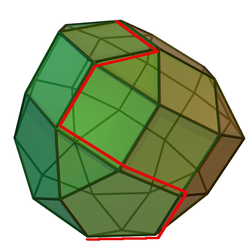
\includegraphics[width=\linewidth, keepaspectratio]{figs/250px-Simplex-method-3-dimensions.png}
      {\scriptsize \textit{Source: Wikipedia / Simplex method in 3D}}
    \end{column}
    
    % === RIGHT: Text ===
    \begin{column}{0.52\textwidth}
      \textbf{Core Idea:}
      \begin{itemize}%[leftmargin=*, nosep]
        \item Exploit problem geometry in primal \& dual space
        \item Navigate along vertices of the feasible polyhedron
        \item Each pivot moves to a better adjacent vertex
      \end{itemize}
      
      \vspace{0.3cm}
      \textbf{How Simplex Works:}
      \begin{itemize}%[leftmargin=*, nosep]
        \item Starts at a feasible vertex
        \item Pivots to adjacent vertex with better objective
        \item Stops at optimum (no improving neighbor)
      \end{itemize}
      
      \vspace{0.3cm}
      \textbf{Related Methods:}
      \begin{itemize}%[leftmargin=*, nosep]
        \item Dantzig algorithm (original simplex)
        \item Russell algorithm (simpler variant)
      \end{itemize}
    \end{column}
  \end{columns}
\end{frame}





%%%%%%%%%%%%%%%%%%%%%%%%%%%%%%%%%%%%%%
\begin{frame}{Simplex Algorithm and Tableau}
\footnotesize

\begin{columns}[T]
  % === LEFT COLUMN: Primal + Dual ===
  \begin{column}{0.48\textwidth}
    \textbf{Primal (Max):}
    \[
      \scriptsize
      \begin{aligned}
        \max \quad & Z = c_1 x_1 + c_2 x_2 \\
        \text{s.t.} \quad & a_{11}x_1 + a_{12}x_2 \leq b_1 \\
                          & a_{21}x_1 + a_{22}x_2 \leq b_2 \\
                          & x_1, x_2 \geq 0
      \end{aligned}
    \]

    \vspace{0.15cm}
    \hrule height 0.2pt
    \vspace{0.15cm}

    \textbf{Dual (Min):}
    \[
      \scriptsize
      \begin{aligned}
        \min \quad & W = b_1 y_1 + b_2 y_2 \\
        \text{s.t.} \quad & a_{11}y_1 + a_{21}y_2 \geq c_1 \\
                          & a_{12}y_1 + a_{22}y_2 \geq c_2 \\
                          & y_1, y_2 \geq 0
      \end{aligned}
    \]

    \vspace{0.2cm}
    {\scriptsize \textit{Intro resource: }
    \href{https://www.matem.unam.mx/~omar/math340/simplex-intro.html}{\texttt{matem.unam.mx/simplex-intro}}}
  \end{column}

  % === RIGHT COLUMN: Simplex Tableau ===
  \begin{column}{0.52\textwidth}
    \textbf{Initial Simplex Tableau:}
    \[
      \scriptsize
      \renewcommand{\arraystretch}{1.1}
      \begin{array}{c|cccc|c}
        \text{BV} & x_1 & x_2 & s_1 & s_2 & \text{RHS} \\
        \hline
        s_1 & a_{11} & a_{12} & 1 & 0 & b_1 \\
        s_2 & a_{21} & a_{22} & 0 & 1 & b_2 \\
        \hline
        Z   & -c_1 & -c_2 & 0 & 0 & 0
      \end{array}
    \]

    \vspace{0.2cm}
    {\scriptsize
    \textbf{How Simplex Works:}
    \begin{itemize}
      \item Starts at feasible vertex (slacks $s_1, s_2$)
      \item Pivots to adjacent vertex with better objective
      \item \textbf{Pivot rule}: Most negative in $Z$-row + min-ratio test
      \item \textbf{Optimal}: All $Z$-row coefficients $\geq 0$
    \end{itemize}}
  \end{column}
\end{columns}

\end{frame}



\begin{frame}{Introduction to Simplex Tableau}
    \small
    \textbf{Tutorials}
    \begin{itemize}
        \item \href{https://vijayasriiyer.medium.com/simplex-method-the-easy-way-f19e61095ac7}{\underline{Simplex Method the Easy Way}} \\
        \textit{(intuitive step-by-step guide)}
        \item \href{https://www.columbia.edu/~cs2035/courses/ieor3608.F02/tableaunotes2.pdf}{\underline{Columbia IEOR: Tableau Notes (PDF)}} \\
        \textit{(formal tableau mechanics \& pivot rules)}
    \end{itemize}
    
    \vspace{0.3cm}
    \textbf{Videos}
    \begin{itemize}
        \item \href{https://www.youtube.com/watch?v=VbQU59a4XxA}{\underline{Simplex Algorithm: Pivoting}} \\
        \textit{(mathematical derivation)}
        \item \href{https://www.youtube.com/watch?v=9YKLXFqCy6E}{\underline{Tableau and Pivot (Practical)}} \\
        \textit{(hands-on walkthrough)}
        \item \href{https://www.youtube.com/watch?v=E72DWgKP_1Y}{\underline{The Art of Linear Programming}} \\
        \textit{(conceptual overview)}
    \end{itemize}
\end{frame}


\end{document}

